\documentclass[letterpaper,10pt]{book}
% Change to 10 pt
\usepackage{pdfpages}
\usepackage{morewrites}			% to counteract the no write space problem
\setcounter{tocdepth}{6}

\usepackage[framemethod=TikZ]{mdframed}

\usepackage{fancyhdr}

\usepackage{paralist}
\usepackage{amsmath}
\usepackage{amsfonts}
\usepackage{amssymb}
\usepackage{graphicx}

\usepackage{datetime}
%\usepackage{ulem}

%\usepackage[nottoc]{toobibind}

\usepackage[inline]{enumitem}

% Outer margin at 2.50 is exacty correct to fit the ``corruption alert'' tables
\usepackage[inner=1.0in, outer=2.50in, top=2.54cm,bottom=2.54cm, marginparwidth=2.25in]{geometry}

\usepackage{marginnote}
\usepackage{longtable}
\usepackage{booktabs}
\usepackage{xcolor}

\usepackage{soul}

%%%%%%%%%%%%
\definecolor{ForestGreen}{rgb}{0.00,0.29,0.098}
%%%%%%%%%%%%

\usepackage{marginnote}

\usepackage{imakeidx} 
\usepackage[
	backref=true,
	style=numeric,
%	citestyle=numeric,
	backend=bibtex
	]{biblatex}
\usepackage[driverfallback=hypertex,colorlinks=True]{hyperref}
\usepackage{cleveref}

\makeindex[name=scripture,columnsep=20pt, columnseprule=True,columns=3, title=Scripture References]
\makeindex[name=speaker,columnsep=20pt, columnseprule=True,,columns=2, title=Sermon Creator]
\makeindex[name=series,columnsep=20pt, columnseprule=True,,columns=2, title=Sermon Series]
\makeindex[name=date,columnsep=20pt, columnseprule=True,columns=2, title=Sermon Date]
\makeindex[name=event,columnsep=20pt, columnseprule=True,columns=2, title=Event]
\makeindex[name=topic,columnsep=20pt, columnseprule=True,columns=2, title=Topic]
\makeindex[name=AWIP,columnsep=20pt, columnseprule=True,columns=3, title=All Words in Passage]
\makeindex[name=NWIV,columnsep=20pt, columnseprule=True,columns=3, title=Number of Words in Verse]
\makeindex[name=PNIP,columnsep=20pt, columnseprule=True,columns=3, title=Proper Names in Passage]
\makeindex[name=PEIP,columnsep=20pt, columnseprule=True,columns=2, title=Prophetic Events in Passage]
\makeindex[name=TWPAQ,columnsep=20pt, columnseprule=True,columns=1, title=13-Word Phrases and Quotes]
\makeindex[name=PFTTIS,columnsep=20pt, columnseprule=False,columns=3, title=Phrases found 13 times in scripture]
\makeindex[name=WFTTIS,columnsep=20pt, columnseprule=False,columns=3, title=Words found 13 times in scripture]
\makeindex[name=WFITV,columnsep=20pt, columnseprule=False,columns=3, title=Words found in exactly 13 verses]
\makeindex[name=EVENTS,columnsep=20pt, columnseprule=False,columns=2, title=Sermon Log by Place]
\makeindex[name=QUESTIONS,columnsep=20pt, columnseprule=False,columns=2, title=Bible Questions]
\makeindex[name=DOCTRINES,columnsep=20pt, columnseprule=False,columns=2, title=Doctrines]
\makeindex[name=SONGS,columnsep=20pt, columnseprule=False,columns=1, title=Songs]
\makeindex[name=LOCATION,columnsep=20pt, columnseprule=False,columns= 2, title=Location]
\makeindex[name=FACEBOOK,columnsep=20pt, columnseprule=False,columns=2, title=Facebook]
\makeindex[name=DEVOTIONAL,columnsep=20pt, columnseprule=False,columns=2, title=Devotional Items]
%%%%%%%%%%%%%%%%% EXTRA COLORS
\definecolor{champagne}{rgb}{0.97,0.91,0.81}
\definecolor{bone}{rgb}{0.89,0.85,0.79}
\pagestyle{fancy}
\fancyhf{}
\fancyhead[LE,RO]{\today}
\fancyhead[RE,LO]{Daily Bible Reading}
\fancyhead[CE,CO]{-page \thepage  - }

\fancyfoot[CO,CE]{\leftmark}
%\fancyfoot[LE,RO]{CSCE 692, HW1}

\title{DBR\\
Daily \\ Reads}
\author{Keith Anthony \\
\today }
%+/ffffff +   \pagenumbering{gobble}
\bibliography{Bibliographies/All20220122}

\setlength{\fboxsep}{1.0pt}

\usepackage[utf8]{inputenc}
\usepackage{tikz}

\begin{document}
%%%%%%%%%%%% Tile Page

\begin{titlepage}

\begin{flushright}
\rightskip=-2.5cm
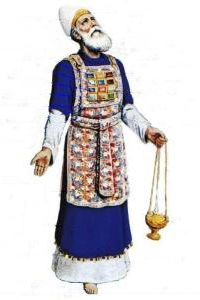
\includegraphics[width=50mm,scale=1.5]{Extras/Melchisedec.jpg}
\vspace{0.4in}  % Create a title for the document and write it in bold font
\LARGE{\textbf{\date}} % Again, do a line break
\linebreak 
% Create a subtitle \large{with Outlines, Statistics, Cross References, and Notes}
\vspace{0.5in}
\begin{flushleft}
\LARGE{Day \#76: Thursday, 17  March 2022 PLAIN  \\}\vspace{0.25in}
\LARGE{Judges 10-12 Psalm 76 Proverb 17}
\end{flushleft}
\vspace{0.6in}
\bigskip

\normalsize{Xenia, Oh.\\}
\normalsize{created: \today}
\vspace{1.3in}

\end{flushright}
\end{titlepage}

\newpage 
\tableofcontents\hypertarget{TOC}{}
\listoffigures
\listoftables

\hyphenation{A-bim-e-lech bre-thren E-phra-im  Gib-e-o-nites Jer-u-sa-lem through-out Phil-i-stines The-o-phil-us Am-a-le-kites ven-geance Mesh-el-e-mi-ah onan-ism Phar-a-oh thoughts grev-ous-ness Hach-a-liah adul-ter-er Shad-rach}

%%%%%%%%%%%%%%%%% EXTRA COLORS
%%%%%%%%%%%%%%%%% EXTRA COLORS
%%%%%%%%%%%%%%%%% EXTRA COLORS
\definecolor{champagne}{rgb}{0.97,0.91,0.81}
\definecolor{bone}{rgb}{0.89,0.85,0.79}

\definecolor{ForestGreen}{rgb}{0.00,0.29,0.098}
\definecolor{GIVING}{cmyk}{1,0.0,0.72,.1}

\definecolor{MLPE}{cmyk}{1,1,0,.45}
\definecolor{SOCCER}{cmyk}{.77, 0, .42, .49}
\definecolor{PAYBILL}{cmyk}{0,0.83,0.76,0.07}
\definecolor{SERMON}{cmyk}{.14,.9,0,.30} % aka seance \href{http://www.flatuicolorpicker.com/purple-cmyk-color-model/}{seance}
\definecolor{BIBLE}{cmyk}{0,.17,.74,.17}
\definecolor{WORKBLUE}{cmyk}{1, .5, 0, .6}
\definecolor{myOrange}{cmyk}{0, .4, .98, .03}
\definecolor{myTan}{cmyk}{0.0,.07,.17,.10}
\definecolor{myRed}{cmyk}{0,1,1,0}
\definecolor{myWhite}{cmyk}{0,0,0,0}
\definecolor{BLUESoD}{cmyk}{.97,.84,0,.04}
\definecolor{WHITE}{cmyk}{0,0,0,0}
\definecolor{OLDGOLD}{cmyk}{0.05,0.3,1.00,0}
\definecolor{CASTLETON}{cmyk}{1,0,0.31,0.66}
\definecolor{cadmiumgreen}{rgb}{0.0, 0.42, 0.24}
\definecolor{jungle}{rgb}{0.203,0.4882,0.1718}
\definecolor{MYGOLD}{rgb}{1,.84,0}

\definecolor{MYLIGHTGRAY}{rgb}{.85,.85,.85}

\definecolor{codegreen}{rgb}{0,0.6,0}
\definecolor{codegray}{rgb}{0.5,0.5,0.5}
\definecolor{codepurple}{rgb}{0.58,0,0.82}
\definecolor{backcolour}{rgb}{0.95,0.95,0.92}


\mdfdefinestyle{MyFrame}{%
    linecolor=blue,
    outerlinewidth=2pt,
    roundcorner=5pt,
    innertopmargin=\baselineskip,
    innerbottommargin=\baselineskip,
    innerrightmargin=10pt,
    innerleftmargin=10pt,
    backgroundcolor=gray!25!white}


\mdfdefinestyle{MyFrame2}{%
    linecolor=black,
    outerlinewidth=2pt,
    roundcorner=5pt,
    innertopmargin=\baselineskip,
    innerbottommargin=\baselineskip,
    innerrightmargin=10pt,
    innerleftmargin=10pt,
    backgroundcolor=yellow!25!white}


%%%%%
%% for PFTTIS list
%%%%%

%%% And Joseph said unto
\index[PFTTIS]{And Joseph said unto!Genesis!Gen 40:008}
\index[PFTTIS]{And Joseph said unto!Genesis!Gen 40:012}
\index[PFTTIS]{And Joseph said unto!Genesis!Gen 41:025}
\index[PFTTIS]{And Joseph said unto!Genesis!Gen 42:014}
\index[PFTTIS]{And Joseph said unto!Genesis!Gen 42:018}
\index[PFTTIS]{And Joseph said unto!Genesis!Gen 44:015}
\index[PFTTIS]{And Joseph said unto!Genesis!Gen 45:003}
\index[PFTTIS]{And Joseph said unto!Genesis!Gen 45:004}
\index[PFTTIS]{And Joseph said unto!Genesis!Gen 46:031}
\index[PFTTIS]{And Joseph said unto!Genesis!Gen 48:009}
\index[PFTTIS]{And Joseph said unto!Genesis!Gen 48:018}
\index[PFTTIS]{And Joseph said unto!Genesis!Gen 50:019}
\index[PFTTIS]{And Joseph said unto!Genesis!Gen 50:024}


%%% a shadow
\index[PFTTIS]{a shadow!1Chronicles!1Chr 029:15}
\index[PFTTIS]{a shadow!Job!Job 008:09}
\index[PFTTIS]{a shadow!Job!Job 014:02}
\index[PFTTIS]{a shadow!Job!Job 017:07}
\index[PFTTIS]{a shadow!Psalm!Psa 102:011}
\index[PFTTIS]{a shadow!Psalm!Psa 144:004}
\index[PFTTIS]{a shadow!Ecclesiastes!Eccl 006:012}
\index[PFTTIS]{a shadow!Ecclesiastes!Eccl 008:013}
\index[PFTTIS]{a shadow!Isaiah!Isa 04:006}
\index[PFTTIS]{a shadow!Isaiah!Isa 25:004}
\index[PFTTIS]{a shadow!Jonah!Jnh 04:06}
\index[PFTTIS]{a shadow!Colossians!Col 02:017}
\index[PFTTIS]{a shadow!Hebews!Heb 10:001}

%%% blessed is the man
\index[PFTTIS]{blessed is the man!Psalm!Psa 001:001}
\index[PFTTIS]{blessed is the man!Psalm!Psa 032:002}
\index[PFTTIS]{blessed is the man!Psalm!Psa 034:008}
\index[PFTTIS]{blessed is the man!Psalm!Psa 065:004}
\index[PFTTIS]{blessed is the man!Psalm!Psa 084:005}
\index[PFTTIS]{blessed is the man!Psalm!Psa 084:012}
\index[PFTTIS]{blessed is the man!Psalm!Psa 094:012}
\index[PFTTIS]{blessed is the man!Psalm!Psa 112:001}
\index[PFTTIS]{blessed is the man!Proverbs!Pro 008:034}
\index[PFTTIS]{blessed is the man!Isaiah!Isa 056:002}
\index[PFTTIS]{blessed is the man!Jeremiah!Jer 017:007}
\index[PFTTIS]{blessed is the man!Romans!Rom 004:008}
\index[PFTTIS]{blessed is the man!James!Jam 001:012}


%%% carry them
\index[PFTTIS]{carry them!Leviticus!Lev 14:045}
\index[PFTTIS]{carry them!Numbers!Num 11:012}
\index[PFTTIS]{carry them!Joshua!Jsh 04:003}
\index[PFTTIS]{carry them!1Samuel!1Sam 20:040}
\index[PFTTIS]{carry them!1Kings!1Kng 08:046}
\index[PFTTIS]{carry them!2Chronicles!2Chr 06:036}
\index[PFTTIS]{carry them!Ezra!Ezra 05:015}
\index[PFTTIS]{carry them!Isaiah!Isa 40:011}
\index[PFTTIS]{carry them!Isaiah!Isa 41:016}
\index[PFTTIS]{carry them!Isaiah!Isa 57:013}
\index[PFTTIS]{carry them!Jeremiah!Jer 20:004}
\index[PFTTIS]{carry them!Jeremiah!Jer 20:005}
\index[PFTTIS]{carry them!Jeremiah!Jer 43:012}


\index[PFTTIS]{good tidings!2Samuel!2Sam 18:027}
\index[PFTTIS]{good tidings!1Kings!1Ki 01:042}
\index[PFTTIS]{good tidings!2Kings!2Ki 07:009 (2x)}
\index[PFTTIS]{good tidings!Isaiah!Isa 40:009 (2x)}
\index[PFTTIS]{good tidings!Isaiah!Isa 41:007}
\index[PFTTIS]{good tidings!Isaiah!Isa 52:007}
\index[PFTTIS]{good tidings!Isaiah!Isa 61:001}
\index[PFTTIS]{good tidings!Nahum!Nah 01:005}
\index[PFTTIS]{good tidings!Luke!Lk 02:010}
\index[PFTTIS]{good tidings!1Thessalonians!1Thess 03:006}


%%% dead body
\index[PFTTIS]{dead body!Leviticus!Lev 21:011}
\index[PFTTIS]{dead body!Numbers!Num 06:006}
\index[PFTTIS]{dead body!Numbers!Num 09:006}
\index[PFTTIS]{dead body!Numbers!Num 09:007}
\index[PFTTIS]{dead body!Numbers!Num 09:010}
\index[PFTTIS]{dead body!Numbers!Num 09:011}
\index[PFTTIS]{dead body!Numbers!Num 09:013}
\index[PFTTIS]{dead body!Numbers!Num 09:016}
\index[PFTTIS]{dead body!2Kings!2Ki 08:005}
\index[PFTTIS]{dead body!Isaiah!Isa 26:019}
\index[PFTTIS]{dead body!Jeremiah!Jer 26:023}
\index[PFTTIS]{dead body!Jeremiah!Jer 36:030}
\index[PFTTIS]{dead body!Haggai!Hag 02:013}

%%% great sea
\index[PFTTIS]{great sea!Numbers!Num 34:006}
\index[PFTTIS]{great sea!Numbers!Num 34:007}
\index[PFTTIS]{great sea!Joshua!Jos 01:004}
\index[PFTTIS]{great sea!Joshua!Jos 09:001}
\index[PFTTIS]{great sea!Joshua!Jos 15:012}
\index[PFTTIS]{great sea!Joshua!Jos 15:047}
\index[PFTTIS]{great sea!Joshua!Jos 23:004}
\index[PFTTIS]{great sea!Ezekiel!Eze 47:010}
\index[PFTTIS]{great sea!Ezekiel!Eze 47:015}
\index[PFTTIS]{great sea!Ezekiel!Eze 47:019}
\index[PFTTIS]{great sea!Ezekiel!Eze 47:020}
\index[PFTTIS]{great sea!Ezekiel!Eze 48:028}
\index[PFTTIS]{great sea!Daniel!Dan 07:002}


%%% have forsaken me
\index[PFTTIS]{have forsaken me!Judges!Jdg 10:013}
\index[PFTTIS]{have forsaken me!1Samuel!1Sam 08:008}
\index[PFTTIS]{have forsaken me!1Kings!1Ki 11:033}
\index[PFTTIS]{have forsaken me!2Kings!2Ki 22:017}
\index[PFTTIS]{have forsaken me!2Chronicles!2Chr 12:005}
\index[PFTTIS]{have forsaken me!2Chronicles!2Chr 34:025}
\index[PFTTIS]{have forsaken me!Jeremiah!Jer 01:016}
\index[PFTTIS]{have forsaken me!Jeremiah!Jer 02:013}
\index[PFTTIS]{have forsaken me!Jeremiah!Jer 05:007}
\index[PFTTIS]{have forsaken me!Jeremiah!Jer 05:019}
\index[PFTTIS]{have forsaken me!Jeremiah!Jer 16:011 (2x)}
\index[PFTTIS]{have forsaken me!Jeremiah!Jer 19:004}

%%% no king
\index[PFTTIS]{no king!Judges!Jdg 17:06}
\index[PFTTIS]{no king!Judges!Jdg 18:01}
\index[PFTTIS]{no king!Judges!Jdg 19:01}
\index[PFTTIS]{no king!Judges!Jdg 21:25}
\index[PFTTIS]{no king!1Kings!1Ki 22:47}
\index[PFTTIS]{no king!2Kings!2Ki 23:25}
\index[PFTTIS]{no king!Nehemiah!Neh 13:26}
\index[PFTTIS]{no king!Psalms!Psa 033:016}
\index[PFTTIS]{no king!Proverbs!Pro 30:27}
\index[PFTTIS]{no king!Daniel!Dan 02:10}
\index[PFTTIS]{no king!Hosea!Hos 10:03}
\index[PFTTIS]{no king!Micah!Mic 04:09}
\index[PFTTIS]{no king!John!Jhn 19:15}


%%% rebellious house
\index[PFTTIS]{rebellious house!Exodus!Exo 02:005}
\index[PFTTIS]{rebellious house!Exodus!Exo 02:006}
\index[PFTTIS]{rebellious house!Exodus!Exo 02:008}
\index[PFTTIS]{rebellious house!Exodus!Exo 03:009}
\index[PFTTIS]{rebellious house!Exodus!Exo 03:026}
\index[PFTTIS]{rebellious house!Exodus!Exo 03:027}
\index[PFTTIS]{rebellious house!Exodus!Exo 12:002 (2x)}
\index[PFTTIS]{rebellious house!Exodus!Exo 12:003}
\index[PFTTIS]{rebellious house!Exodus!Exo 12:009}
\index[PFTTIS]{rebellious house!Exodus!Exo 12:025}
\index[PFTTIS]{rebellious house!Exodus!Exo 17:012}
\index[PFTTIS]{rebellious house!Exodus!Exo 24:003}

%%% seek him
\index[PFTTIS]{seek him!Deuteronomy!Deu 04:029}\index[PFTTIS]{seek him!1Samuel!1Sam 23:025}
\index[PFTTIS]{seek him!1Chronicles!1Chr 28:009}
\index[PFTTIS]{seek him!2Chronicles!1Chr 15:002}
\index[PFTTIS]{seek him!Ezra!Ezr 08:022}
\index[PFTTIS]{seek him!Psalms!Psa 022:026}
\index[PFTTIS]{seek him!Psalms!Psa 024:006}
\index[PFTTIS]{seek him!Psalms!Psa 119:002}
\index[PFTTIS]{seek him!SoS!SoS 03:002}
\index[PFTTIS]{seek him!SoS!SoS 06:001}
\index[PFTTIS]{seek him!Hosea!Hos 07:010}
\index[PFTTIS]{seek him!Amos!Amo 05:008}
\index[PFTTIS]{seek him!Hebrews!Heb 11:0063}


%%% seek ye
\index[PFTTIS]{seek ye!Isaiah!Isa 34:016}
\index[PFTTIS]{seek ye!Isaiah!Isa 45:019}
\index[PFTTIS]{seek ye!Isaiah!Isa 55:006}
\index[PFTTIS]{seek ye!Amos!Amos 5:004}
\index[PFTTIS]{seek ye!John!John 1:38}
\index[PFTTIS]{seek ye!John!John 18:4}
\index[PFTTIS]{seek ye!John!John 18:7}
\index[PFTTIS]{seek ye!Matthew!Matt 6:33}
\index[PFTTIS]{seek ye!Numbers!Num 16:10}
\index[PFTTIS]{seek ye!Luke!Luke 12:31}
\index[PFTTIS]{seek ye!Luke!Luke 24:5}
\index[PFTTIS]{seek ye!Psalm!Psa 27:8}
\index[PFTTIS]{seek ye!Zephaniah!Zeph 2:3}

%%% the uncircumcised
\index[PFTTIS]{the uncircumcised!Genesis!Gen 17:014}
\index[PFTTIS]{the uncircumcised!Judges!Jdg 14:003}
\index[PFTTIS]{the uncircumcised!Judges!Jdg 15:018}
\index[PFTTIS]{the uncircumcised!2Samuel!2Sam 01:020}
\index[PFTTIS]{the uncircumcised!Isaiah!Isa 02:001}
\index[PFTTIS]{the uncircumcised!Jeremiah!Jer 09:025}
\index[PFTTIS]{the uncircumcised!Ezekiel!Eze 28:010}
\index[PFTTIS]{the uncircumcised!Ezekiel!Eze 31:018}
\index[PFTTIS]{the uncircumcised!Ezekiel!Eze 32:019}
\index[PFTTIS]{the uncircumcised!Ezekiel!Eze 32:027}
\index[PFTTIS]{the uncircumcised!Ezekiel!Eze 32:028}
\index[PFTTIS]{the uncircumcised!Ezekiel!Eze 32:029}
\index[PFTTIS]{the uncircumcised!Ezekiel!Eze 32:032}

%%% worship him
\index[PFTTIS]{worship him!Psalms!Psa 97:007}
\index[PFTTIS]{worship him!Zephaniah!Zeph 02:011}
\index[PFTTIS]{worship him!Matthew!Matt 02:002}
\index[PFTTIS]{worship him!Matthew!Matt 02:008}
\index[PFTTIS]{worship him!John!John 04:023}
\index[PFTTIS]{worship him!John!John 04:024 (2x)} 
\index[PFTTIS]{worship him!Acts!Acts 17:023}
\index[PFTTIS]{worship him!Hebrews!Heb 01:006}
\index[PFTTIS]{worship him!Revelation!Rev 04:010}
\index[PFTTIS]{worship him!Revelation!Rev 13:008}
\index[PFTTIS]{worship him!Revelation!Rev 14:007}
\index[PFTTIS]{worship him!Revelation!Rev 19:010}


%%%%%
%% for PFTTIS list
%%%%%

%%% afflictions
\index[WFTTIS]{afflictions!Psalms!Psa 34:019}
\index[WFTTIS]{afflictions!Psalms!Psa 132:001}
\index[WFTTIS]{afflictions!Acts!Acts 07:010}
\index[WFTTIS]{afflictions!Acts!Acts 20:023}
\index[WFTTIS]{afflictions!2Corinthians!2Cor 06:004}
\index[WFTTIS]{afflictions!Colossians!Col 01:024}
\index[WFTTIS]{afflictions!1Thessalonians!1Thess 03:003}
\index[WFTTIS]{afflictions!2Timothy!2Tim 01:008}
\index[WFTTIS]{afflictions!2Timothy!2Tim 03:011}
\index[WFTTIS]{afflictions!2Timothy!2Tim 04:005}
\index[WFTTIS]{afflictions!Hebrews!Heb 10:032}
\index[WFTTIS]{afflictions!Hebrews!Heb 10:033}
\index[WFTTIS]{afflictions!1Peter!1Pet 05:009}

%%% acsend
\index[WFTTIS]{acsend!Joshua!Jos 06:05}
\index[WFTTIS]{acsend!Psalm!Psa 024:003}
\index[WFTTIS]{acsend!Psalm!Psa 135:007}
\index[WFTTIS]{acsend!Psalm!Psa 139:008}
\index[WFTTIS]{acsend!Isaiah!Isa 14:013}
\index[WFTTIS]{acsend!Isaiah!Isa 14:014}
\index[WFTTIS]{acsend!Jeremiah!Jer 10:013}
\index[WFTTIS]{acsend!Jeremiah!Jer 51:016}
\index[WFTTIS]{acsend!Ezekiel!Eze 38:009}
\index[WFTTIS]{acsend!John!John 06:062}
\index[WFTTIS]{acsend!John!John 20:017}
\index[WFTTIS]{acsend!Romans!Rom 10:006}
\index[WFTTIS]{acsend!Revelation!Rev 17:008}

%%% Assyrian
\index[WFTTIS]{Assyrian!Isaiah!Isa 10:005}
\index[WFTTIS]{Assyrian!Isaiah!Isa 10:024}
\index[WFTTIS]{Assyrian!Isaiah!Isa 14:025}
\index[WFTTIS]{Assyrian!Isaiah!Isa 19:023}
\index[WFTTIS]{Assyrian!Isaiah!Isa 23:013}
\index[WFTTIS]{Assyrian!Isaiah!Isa 30:031}
\index[WFTTIS]{Assyrian!Isaiah!Isa 31:008}
\index[WFTTIS]{Assyrian!Isaiah!Isa 52:004}
\index[WFTTIS]{Assyrian!Ezekiel!Eze 31:003}
\index[WFTTIS]{Assyrian!Hosea!Hos 05:013}
\index[WFTTIS]{Assyrian!Hosea!Hos 11:005}
\index[WFTTIS]{Assyrian!Micah!Hos 05:005}
\index[WFTTIS]{Assyrian!Micah!Hos 05:006}

%%% blot
\index[WFTTIS]{blot!Exodus!Exo 32:032}
\index[WFTTIS]{blot!Exodus!Exo 32:033}
\index[WFTTIS]{blot!Numbers!Num 05:026}
\index[WFTTIS]{blot!Deuteronomy!Deut 09:014}
\index[WFTTIS]{blot!Deuteronomy!Deut 25:019}
\index[WFTTIS]{blot!Deuteronomy!Deut 29:020}
\index[WFTTIS]{blot!2Kings!2Ki 14:027}
\index[WFTTIS]{blot!Job!Job 31:007}
\index[WFTTIS]{blot!Psalms!Psa 51:001}
\index[WFTTIS]{blot!Psalms!Psa 51:009}
\index[WFTTIS]{blot!Proverbs!Pro 09:007}
\index[WFTTIS]{blot!Jeremiah!Jer 18:023}
\index[WFTTIS]{blot!Revelation!Rev 03:005}


%%% chain
\index[WFTTIS]{chain!Genesis!Gen 41:042}
\index[WFTTIS]{chain!1Kings!1Ki 07:017}
\index[WFTTIS]{chain!Psalms!Psa 73:006}
\index[WFTTIS]{chain!SoS!Sos 04:009}
\index[WFTTIS]{chain!Lamentations!Lam 03:007}
\index[WFTTIS]{chain!Ezekiel!Eze 07:023}
\index[WFTTIS]{chain!Ezekiel!Eze 16:011}
\index[WFTTIS]{chain!Daniel!Dan 05:007}
\index[WFTTIS]{chain!Daniel!Dan 05:016}
\index[WFTTIS]{chain!Daniel!Dan 05:029}
\index[WFTTIS]{chain!Acts!Acts 28:020}
\index[WFTTIS]{chain!2Timothy!2Tim 01:016}
\index[WFTTIS]{chain!Revelation!Rev 20:001}


%%% controversy
\index[WFTTIS]{controversy!Deuteronomy!Deu 17:008}
\index[WFTTIS]{controversy!Deuteronomy!Deu 19:017}
\index[WFTTIS]{controversy!Deuteronomy!Deu 21:005}
\index[WFTTIS]{controversy!Deuteronomy!Deu 25:001}
\index[WFTTIS]{controversy!2Samuel!2Sam 15:002}
\index[WFTTIS]{controversy!Isaiah!Isa 34:008}
\index[WFTTIS]{controversy!Jeremiah!Jer 25:031}
\index[WFTTIS]{controversy!Ezekiel!Eze 44:024}
\index[WFTTIS]{controversy!Hosea!Hos 04:001}
\index[WFTTIS]{controversy!Hosea!Hos 12:002}
\index[WFTTIS]{controversy!Micah!Mic 06:002 (2x)}
\index[WFTTIS]{controversy!1Timothy!1Tim 03:016}


%%% Dagon/Dagon's
\index[WFTTIS]{Dagon!Judges!Jdg 16:023}
\index[WFTTIS]{Dagon!1Samuel!1Sam 05:002 (2x)}
\index[WFTTIS]{Dagon!1Samuel!1Sam 05:003 (2x)}
\index[WFTTIS]{Dagon!1Samuel!1Sam 05:004 (3x)}
\index[WFTTIS]{Dagon!1Samuel!1Sam 05:005 (3x)}
\index[WFTTIS]{Dagon!1Samuel!1Sam 05:007}
\index[WFTTIS]{Dagon!1Chronicles!1Chr 10:010}

%%% disobedient
\index[WFTTIS]{disobedient!1Kings!1Ki 13:026}
\index[WFTTIS]{disobedient!Nehemiah!Neh 09:026}
\index[WFTTIS]{disobedient!Luke!Luke 01:017}
\index[WFTTIS]{disobedient!Acts!Acts 26:019}
\index[WFTTIS]{disobedient!Romans!Rom 01:030}
\index[WFTTIS]{disobedient!Romans!Rom 10:021}
\index[WFTTIS]{disobedient!1Timothy!1Tim 01:009}
\index[WFTTIS]{disobedient!2Timothy!2Tim 03:002}
\index[WFTTIS]{disobedient!Titus!Titus 01:016}
\index[WFTTIS]{disobedient!Titus!Titus 03:003}
\index[WFTTIS]{disobedient!1Peter!1Pet 02:007}
\index[WFTTIS]{disobedient!1Peter!1Pet 02:008}
\index[WFTTIS]{disobedient!1Peter!1Pet 03:020}


%%% doubt
\index[WFTTIS]{doubt!Genesis!Gen 37:033}
\index[WFTTIS]{doubt!Deuteronomy!Deu 28:066}
\index[WFTTIS]{doubt!Job!Job 12:002}
\index[WFTTIS]{doubt!Matthew!Matt 14:031}
\index[WFTTIS]{doubt!Matthew!Matt 21:021}
\index[WFTTIS]{doubt!Mark!Mk 11:023}
\index[WFTTIS]{doubt!Luke!Lk 11:020}
\index[WFTTIS]{doubt!John!Jhn 10:024}
\index[WFTTIS]{doubt!Acts!Acts 02:012}
\index[WFTTIS]{doubt!Acts!Acts 28:004}
\index[WFTTIS]{doubt!1Corinthians!1Cor 09:010}
\index[WFTTIS]{doubt!Galatians!Gal 04:020}
\index[WFTTIS]{doubt!1John!1Jhn 02:019}


%%% dungeon
\index[WFTTIS]{dungeon!Genesis!Gen 40:015}
\index[WFTTIS]{dungeon!Genesis!Gen 41:014}
\index[WFTTIS]{dungeon!Exodus!Exo 12:029}
\index[WFTTIS]{dungeon!Jeremiah!Jer 37:016}
\index[WFTTIS]{dungeon!Jeremiah!Jer 38:006 (2x)}
\index[WFTTIS]{dungeon!Jeremiah!Jer 38:007}
\index[WFTTIS]{dungeon!Jeremiah!Jer 38:009}
\index[WFTTIS]{dungeon!Jeremiah!Jer 38:010}
\index[WFTTIS]{dungeon!Jeremiah!Jer 38:011}
\index[WFTTIS]{dungeon!Jeremiah!Jer 38:013}
\index[WFTTIS]{dungeon!Lamentations!Lam 03:053}
\index[WFTTIS]{dungeon!Lamentations!Lam 03:055}


%%% error
\index[WFTTIS]{error!2Samuel!2Sam 06:007}
\index[WFTTIS]{error!Job!Job 19:004}
\index[WFTTIS]{error!Ecclesiastes!Ecc 05:006}
\index[WFTTIS]{error!Ecclesiastes!Ecc 10:005}
\index[WFTTIS]{error!Isaiah!Isa 32:006}
\index[WFTTIS]{error!Daniel!Dan 06:004}
\index[WFTTIS]{error!Matthew!Matt 27:064}
\index[WFTTIS]{error!Romans!Rom 01:027}
\index[WFTTIS]{error!James!Jam 05:020}
\index[WFTTIS]{error!2Peter!2Pet 02:018}
\index[WFTTIS]{error!2Peter!2Pet 03:017}
\index[WFTTIS]{error!1John!1Jn 04:006}
\index[WFTTIS]{error!Jude!Jude 01:011}

%%% fourish
\index[WFTTIS]{fourish!Psalms!Psa 072:007}
\index[WFTTIS]{fourish!Psalms!Psa 072:016}
\index[WFTTIS]{fourish!Psalms!Psa 092:007}
\index[WFTTIS]{fourish!Psalms!Psa 092:012}
\index[WFTTIS]{fourish!Psalms!Psa 092:013}
\index[WFTTIS]{fourish!Psalms!Psa 132:018}
\index[WFTTIS]{fourish!Proverbs!Pro 11:28}
\index[WFTTIS]{fourish!Proverbs!Pro 14:11}
\index[WFTTIS]{fourish!Ecclesiastes!Ecc 12:05}
\index[WFTTIS]{fourish!SongOfSolomon!SOS 07:12}
\index[WFTTIS]{fourish!Isaiah!Isa 17:11}
\index[WFTTIS]{fourish!Isaiah!Isa 66:14}
\index[WFTTIS]{fourish!Ezekiel!Eze 17:24}




%%% giants
\index[WFTTIS]{giants!Genesis!Gen 06:004}
\index[WFTTIS]{giants!Numbers!Num 13:033}
\index[WFTTIS]{giants!Deuteronomy!Deut 02:011}
\index[WFTTIS]{giants!Deuteronomy!Deut 02:021}
\index[WFTTIS]{giants!Deuteronomy!Deut 03:011}
\index[WFTTIS]{giants!Deuteronomy!Deut 03:013}
\index[WFTTIS]{giants!Joshua!Josh 12:004}
\index[WFTTIS]{giants!Joshua!Josh 13:012}
\index[WFTTIS]{giants!Joshua!Josh 15:008}
\index[WFTTIS]{giants!Joshua!Josh 17:015}
\index[WFTTIS]{giants!Joshua!Josh 16:016}

%%% good man
\index[WFTTIS]{good man!2 Samuel!2Sa 18:27}
%(1) Psalms 37:23 [5]
%(1) Psalms 112:5 [2]
%(1) Proverbs 12:2 [2]
%(1) Proverbs 13:22 [2]
%(1) Proverbs 14:14 [14]
%(1) Micah 7:2 [2]
%(1) Matthew 12:35 [2]
%(1) Luke 6:45 [2]
%(1) Luke 23:50 [15]
%(1) John 7:12 [17]
%(1) Acts 11:24 [5]
%(1) Romans 5:7 [14]

%%% Hinnom
\index[WFTTIS]{Hinnom!Joshua!Jsh 15:008}
\index[WFTTIS]{Hinnom!Joshua!Jsh 18:016}
\index[WFTTIS]{Hinnom!2Kings!2Ki 23:010}
\index[WFTTIS]{Hinnom!2Chronicles!2Chr 28:003}
\index[WFTTIS]{Hinnom!2Chronicles!2Chr 33:006}
\index[WFTTIS]{Hinnom!Nehemiah!Neh 11:030}
\index[WFTTIS]{Hinnom!Jeremiah!Jer 07:031}
\index[WFTTIS]{Hinnom!Jeremiah!Jer 07:032}
\index[WFTTIS]{Hinnom!Jeremiah!Jer 19:002}
\index[WFTTIS]{Hinnom!Jeremiah!Jer 19:006}
\index[WFTTIS]{Hinnom!Jeremiah!Jer 32:035}

%%% inclined
\index[WFTTIS]{inclined!Judges!Jdg 09:003}
\index[WFTTIS]{inclined!Psalms!Psa 040:001}
\index[WFTTIS]{inclined!Psalms!Psa 116:002}
\index[WFTTIS]{inclined!Psalms!Psa 119:112}
\index[WFTTIS]{inclined!Proverbs!Pro 05:13}
\index[WFTTIS]{inclined!Jeremiah!Jer 07:24}
\index[WFTTIS]{inclined!Jeremiah!Jer 07:26}
\index[WFTTIS]{inclined!Jeremiah!Jer 11:08}
\index[WFTTIS]{inclined!Jeremiah!Jer 17:23}
\index[WFTTIS]{inclined!Jeremiah!Jer 25:04}
\index[WFTTIS]{inclined!Jeremiah!Jer 34:14}
\index[WFTTIS]{inclined!Jeremiah!Jer 35:15}
\index[WFTTIS]{inclined!Jeremiah!Jer 44:05}


%%% laughed
\index[WFTTIS]{laughed!Genesis!Gen 17:017}
\index[WFTTIS]{laughed!Genesis!Gen 18:012}
\index[WFTTIS]{laughed!Genesis!Gen 18:015}
\index[WFTTIS]{laughed!2Kings!2Ki 19:021}
\index[WFTTIS]{laughed!2Chronicles!2Chr 30:010}
\index[WFTTIS]{laughed!Nehemiah!Neh 02:019}
\index[WFTTIS]{laughed!Job!Job 12:004}
\index[WFTTIS]{laughed!Job!Job 29:024}
\index[WFTTIS]{laughed!Isaiah!Isa 37:022}
\index[WFTTIS]{laughed!Ezekiel!Ezek 23:032}
\index[WFTTIS]{laughed!Matthew!Matt 09:024}
\index[WFTTIS]{laughed!Mark!Mk 05:040}
\index[WFTTIS]{laughed!Luke!Lk 08:053}

%%% liar
\index[WFTTIS]{liar!Job!Job 24:025}
\index[WFTTIS]{liar!Proverbs!Pro 17:004}
\index[WFTTIS]{liar!Proverbs!Pro 19:022}
\index[WFTTIS]{liar!Proverbs!Pro 30:006}
\index[WFTTIS]{liar!Jeremiah!Jer 15:018}
\index[WFTTIS]{liar!John!Jhn 08:044}
\index[WFTTIS]{liar!John!Jhn 08:055}
\index[WFTTIS]{liar!Romans!Rom 03:004}
\index[WFTTIS]{liar!1John!1Jhn 01:010}
\index[WFTTIS]{liar!1John!1Jhn 02:004}
\index[WFTTIS]{liar!1John!1Jhn 02:022}
\index[WFTTIS]{liar!1John!1Jhn 04:020}
\index[WFTTIS]{liar!1John!1Jhn 05:010}

%%% palsy
\index[WFTTIS]{palsy!Matthew!Matt 04:024}
\index[WFTTIS]{palsy!Matthew!Matt 08:006}
\index[WFTTIS]{palsy!Matthew!Matt 09:002}
\index[WFTTIS]{palsy!Matthew!Matt 09:006}
\index[WFTTIS]{palsy!Mark!Mk 02:003}
\index[WFTTIS]{palsy!Mark!Mk 02:004}
\index[WFTTIS]{palsy!Mark!Mk 02:005}
\index[WFTTIS]{palsy!Mark!Mk 02:009}
\index[WFTTIS]{palsy!Mark!Mk 02:010}
\index[WFTTIS]{palsy!Luke!Lk 05:018}
\index[WFTTIS]{palsy!Luke!Lk 05:024}
\index[WFTTIS]{palsy!Acts!Acts 09:033}

%%% Profitable
\index[WFTTIS]{profitable!Job!Job 22:002 (2x)}
\index[WFTTIS]{profitable!Ecclesiastes!Ecc 10:010}
\index[WFTTIS]{profitable!Isaiah!Isa 44:010}
\index[WFTTIS]{profitable!Jeremiah!Jer 13:007}
\index[WFTTIS]{profitable!Matthew!Matt 05:029}
\index[WFTTIS]{profitable!Matthew!Matt 05:030}
\index[WFTTIS]{profitable!Acts!Acts 20:020}
\index[WFTTIS]{profitable!1Timothy!1Tim 04:008}
\index[WFTTIS]{profitable!2Timothy!2Tim 03:016}
\index[WFTTIS]{profitable!2Timothy!2Tim 04:011}
\index[WFTTIS]{profitable!Titus!Titus 03:008}
\index[WFTTIS]{profitable!Philemon!Phlm 01:011}

%%% Rechab
\index[WFTTIS]{Rechab!2Samuel!2Sam 04:002}
\index[WFTTIS]{Rechab!2Samuel!2Sam 04:005}
\index[WFTTIS]{Rechab!2Samuel!2Sam 04:006}
\index[WFTTIS]{Rechab!2Samuel!2Sam 04:009}
\index[WFTTIS]{Rechab!2KIngs!2Ki 10:015}
\index[WFTTIS]{Rechab!2KIngs!2Ki 10:023}
\index[WFTTIS]{Rechab!1Chronicles!1Chr 02:055}
\index[WFTTIS]{Rechab!Nehemiah!Neh 03:014}
\index[WFTTIS]{Rechab!Jeremiah!Jer 35:006}
\index[WFTTIS]{Rechab!Jeremiah!Jer 35:008}
\index[WFTTIS]{Rechab!Jeremiah!Jer 35:014}
\index[WFTTIS]{Rechab!Jeremiah!Jer 35:016}
\index[WFTTIS]{Rechab!Jeremiah!Jer 35:019}

%%% serpents
\index[WFTTIS]{serpents!Exodus!Exo 07:012}
\index[WFTTIS]{serpents!Numbers!Num 21:006}
\index[WFTTIS]{serpents!Numbers!Num 21:007}
\index[WFTTIS]{serpents!Deuteronomy!Deu 08:015}
\index[WFTTIS]{serpents!Deuteronomy!Deu 32:024}
\index[WFTTIS]{serpents!Jeremiah!Jer 08:017}
\index[WFTTIS]{serpents!Matthew!Matt 10:016}
\index[WFTTIS]{serpents!Matthew!Matt 23:033}
\index[WFTTIS]{serpents!Mark!Mk 16:018}
\index[WFTTIS]{serpents!Luke!Lk 10:019}
\index[WFTTIS]{serpents!1Corinthians!1Cor 10:009}
\index[WFTTIS]{serpents!James!Jas 03:007}
\index[WFTTIS]{serpents!Revelation!Rev 09:019}

%%% short
\index[WFTTIS]{short!Numbers!Num 11:023}
\index[WFTTIS]{short!2Kings!2Ki 10:032}
\index[WFTTIS]{short!Job!Job 17:012}
\index[WFTTIS]{short!Job!Job 20:005}
\index[WFTTIS]{short!Psalms!Psa 89:047}
\index[WFTTIS]{short!Romans!Rom 03:023}
\index[WFTTIS]{short!Romans!Rom 09:028  (2x)}
\index[WFTTIS]{short!1Corinthians!1Cor 07:029}
\index[WFTTIS]{short!1Thessalonians!1Thess 02:017}
\index[WFTTIS]{short!Hebrews!Heb 04:001}
\index[WFTTIS]{short!Revelation!Rev 12:012}
\index[WFTTIS]{short!Revelation!Rev 17:010}

%%% smiteth
\index[WFTTIS]{smiteth!Exodus!Exo 21:012}
\index[WFTTIS]{smiteth!Exodus!Exo 21:15}
\index[WFTTIS]{smiteth!Deuteronomy!Dt 25:11}
\index[WFTTIS]{smiteth!Deuteronomy!Dt 27:24}
\index[WFTTIS]{smiteth!Joshua!Jsh 15:16}
\index[WFTTIS]{smiteth!Judges!Jdg 15:16}
\index[WFTTIS]{smiteth!2 Samuel!2Sa 05:08}
\index[WFTTIS]{smiteth!1Chronicles!1Chr 11:06}
\index[WFTTIS]{smiteth!Job!1Chr 26:12}
\index[WFTTIS]{smiteth!Isaiah!Isa 09:13}
\index[WFTTIS]{smiteth!Lamentations!Lam 03:30}
\index[WFTTIS]{smiteth!Ezekiel!Eze 07:09}
\index[WFTTIS]{smiteth!Luke!Lk 06:29}



%%% vanities
\index[WFTTIS]{vanities!Deuteronomy!Deut 21:021}
\index[WFTTIS]{vanities!1Kings!1Ki 16:013}
\index[WFTTIS]{vanities!1Kings!1Ki 16:026}
\index[WFTTIS]{vanities!Psalms!Psa 031:006}
\index[WFTTIS]{vanities!Ecclesiastes!Ecc 01:002 (2x)}
\index[WFTTIS]{vanities!Ecclesiastes!Ecc 05:007}
\index[WFTTIS]{vanities!Ecclesiastes!Ecc 12:008}
\index[WFTTIS]{vanities!Jeremiah!Jer 08:019}
\index[WFTTIS]{vanities!Jeremiah!Jer 10:008}
\index[WFTTIS]{vanities!Jeremiah!Jer 14:022}
\index[WFTTIS]{vanities!Jonah!Jnh 02:008}
\index[WFTTIS]{vanities!Acts!Acts 14:015}



%%%%%
%% for PFTTIS list
%%%%%

%%% worm
\index[WFITV]{worm!Exodus!Exo 16:024}
\index[WFITV]{worm!Job!Job 17:014}
\index[WFITV]{worm!Job!Job 24:029}
\index[WFITV]{worm!Job!Job 25:005 (2x)}
\index[WFITV]{worm!Psalms!Psa 022:006}
\index[WFITV]{worm!Isaiah!Isa 14:011}
\index[WFITV]{worm!Isaiah!Isa 41:014}
\index[WFITV]{worm!Isaiah!Isa 51:008}
\index[WFITV]{worm!Isaiah!Isa 66:024}
\index[WFITV]{worm!Jonah!Jnh 04:007}
\index[WFITV]{worm!Mark!Mk 09:044}
\index[WFITV]{worm!Mark!Mk 09:046}
\index[WFITV]{worm!Mark!Mk 09:048}


%\subsubsection{Title}
%\textbf{Introduction:} Isaiah 46 
%\index[speaker]{Speaker!Isaiah 49 (Title}
%\index[series]{Book (Speaker)!IPassage (Title)}
%\index[date]{2017/07/09!Isaiah 49 (Title)}
%\begin{compactenum}[I.]
%    \item  \textbf{Point} \index[scripture]{Isaiah!IPassage} (IPassage)
%\end{compactenum}




  

\chapter{Judges 10}
 %  \textcolor[cmyk]{0.99998,1,0,0}{

\marginpar{\scriptsize \centering \fcolorbox{black}{lime}{\textbf{2$^{nd}$} WAVE OF JUDGES}\\ (Judges 10) \begin{compactenum}[I.][8]
    \item  \textbf{Declining Character} \index[scripture]{Judges!Jdg 10:04}(Jdg 10:4) -- Tola and Jair are famous for wealth, Jephthah and Samson for their failures
    \item  \textbf{Desperate Conditions} \index[scripture]{Judges!Jdg 10:08}(Jdg 10:8)
    \item  \textbf{Despicable Conduct} \index[scripture]{Judges!Jdg 10:06}(Jdg 10:6)
    \item  A \textbf{Dash of Conscience} \index[scripture]{Judges!Jdg 10:15}(Jdg 10:15)
    \item  A \textbf{Deliverance Cry} \index[scripture]{Judges!Jdg 10:15}(Jdg 10:15)
    \item   \textbf{Dismissed Charges} \index[scripture]{Judges!Jdg 10:16}(Jdg 10:16)
    \item  A \textbf{Desired Champion} \index[scripture]{Judges!Jdg 10:18}(Jdg 10:18)
\end{compactenum}}


\footnote{\textcolor[rgb]{0.00,0.25,0.00}{\hyperlink{JudgesTOC}{Return to end of Table of Contents.}}}\footnote{\href{https://audiobible.com/bible/judges_10.html}{\textcolor[cmyk]{0.99998,1,0,0}{Judges 10 Audio}}}\textcolor[cmyk]{0.99998,1,0,0}{And after Abimelech there arose to defend \fcolorbox{bone}{bone}{Israel} Tola the son of Puah, the son of Dodo, a man of Issachar; and he dwelt in Shamir in mount Ephraim.}
[2] \textcolor[cmyk]{0.99998,1,0,0}{And he judged \fcolorbox{bone}{bone}{Israel} twenty and three years, and died, and was buried in Shamir.}\\
\\
\P \textcolor[cmyk]{0.99998,1,0,0}{And after him arose Jair, a Gileadite, and judged \fcolorbox{bone}{bone}{Israel} twenty and two years.}
[4] \textcolor[cmyk]{0.99998,1,0,0}{And he had thirty sons that rode on thirty ass colts, and they had thirty cities, which are called Havoth-jair unto this day, which \emph{are} in the land of Gilead.}\\
\\
\P \textcolor[cmyk]{0.99998,1,0,0}{And Jair died, and was buried in Camon.}
[6] \textcolor[cmyk]{0.99998,1,0,0}{And \fcolorbox{bone}{bone}{the children of} \fcolorbox{bone}{bone}{Israel} did evil again in the sight of the LORD, and served Baalim, and Ashtaroth, and the gods of Syria, and the gods of Zidon, and the gods of Moab, and the gods of \fcolorbox{bone}{bone}{the children of} Ammon, and the gods of the Philistines, and forsook the LORD, and served not him.}
[7] \textcolor[cmyk]{0.99998,1,0,0}{And the anger of the LORD was hot against \fcolorbox{bone}{bone}{Israel}, and he sold them into the hands of the Philistines, and into the hands of \fcolorbox{bone}{bone}{the children of} Ammon.}
[8] \textcolor[cmyk]{0.99998,1,0,0}{And that year they vexed and oppressed \fcolorbox{bone}{bone}{the children of} \fcolorbox{bone}{bone}{Israel}: eighteen years, all \fcolorbox{bone}{bone}{the children of} \fcolorbox{bone}{bone}{Israel} that \emph{were} on the other side Jordan in the land of the Amorites, which \emph{is} in Gilead.}
[9] \textcolor[cmyk]{0.99998,1,0,0}{Moreover \fcolorbox{bone}{bone}{the children of} Ammon passed over Jordan to fight also against Judah, and against Benjamin, and against the house of Ephraim; so that \fcolorbox{bone}{bone}{Israel} was sore distressed.}\\
\\
\P \textcolor[cmyk]{0.99998,1,0,0}{And \fcolorbox{bone}{bone}{the children of} \fcolorbox{bone}{bone}{Israel} cried unto the LORD, saying, We have sinned against thee, both because we have forsaken our God, and also served Baalim.}
[11] \textcolor[cmyk]{0.99998,1,0,0}{And the LORD said unto \fcolorbox{bone}{bone}{the children of} \fcolorbox{bone}{bone}{Israel}, \emph{Did} not \emph{I} \emph{deliver} \emph{you} from the Egyptians, and from the Amorites, from \fcolorbox{bone}{bone}{the children of} Ammon, and from the Philistines?}
[12] \textcolor[cmyk]{0.99998,1,0,0}{The Zidonians also, and the Amalekites, and the Maonites, did oppress you; and ye cried to me, and I delivered you out of their hand.}
[13] \textcolor[cmyk]{0.99998,1,0,0}{Yet ye have forsaken me, and served other gods: wherefore I will deliver you no more.}
[14] \textcolor[cmyk]{0.99998,1,0,0}{Go and cry unto the gods which ye have chosen; let them deliver you in the time of your tribulation.}\\
\\
\P \textcolor[cmyk]{0.99998,1,0,0}{And \fcolorbox{bone}{bone}{the children of} \fcolorbox{bone}{bone}{Israel} said unto the LORD, We have sinned: do thou unto us whatsoever seemeth good unto thee; deliver us only, we pray thee, this day.}
[16] \textcolor[cmyk]{0.99998,1,0,0}{And they put away the strange gods from among them, and served the LORD: and his soul was grieved for the misery of \fcolorbox{bone}{bone}{Israel}.}
[17] \textcolor[cmyk]{0.99998,1,0,0}{Then \fcolorbox{bone}{bone}{the children of} Ammon were gathered together, and encamped in Gilead. And \fcolorbox{bone}{bone}{the children of} \fcolorbox{bone}{bone}{Israel} assembled themselves together, and encamped in Mizpeh.}
[18] \textcolor[cmyk]{0.99998,1,0,0}{And the people \emph{and} princes of Gilead said one to another, What man \emph{is} \emph{he} that will begin to fight against \fcolorbox{bone}{bone}{the children of} Ammon? he shall be head over all the inhabitants of Gilead.}
\chapter{Judges 11}
 %  \textcolor[cmyk]{0.99998,1,0,0}{

\marginpar{\scriptsize \centering \fcolorbox{bone}{lime}{CHOOSING JEPHTHAH}\\ (Judges 11) \begin{compactenum}[I.][8]
    \item  The \textbf{Rejection} \index[scripture]{Judges!Jdg 11:01}(Jdg 11:2) 
    \item  A \textbf{Reputation} \index[scripture]{Judges!Jdg 11:06}(Jdg 11:6) 
    \item  The \textbf{Request} \index[scripture]{Judges!Jdg 11:09}(Jdg 11:9) 
    \item  A Heathen \textbf{Ritual} \index[scripture]{Judges!Jdg 11:31}(Jdg 11:31) 
    \item  The \textbf{Return} \index[scripture]{Judges!Jdg 11:34}(Jdg 11:34) 
    \item  The \textbf{Rending} \index[scripture]{Judges!Jdg 11:35}(Jdg 11:35) 
    \item  The \textbf{Remembrance} \index[scripture]{Judges!Jdg 11:40}(Jdg 11:40) 
\end{compactenum}}

\marginpar{\scriptsize \centering \fcolorbox{bone}{yellow}{JEPHTHAH'S VOW}\\ (Judges 11) \begin{compactenum}[I.][8]
    \item  The \textbf{Rash Vow} \index[scripture]{Judges!Jdg 11:31}(Jdg 11:31) 
    \item  The \textbf{Rash Vow} \index[scripture]{Judges!Jdg 11:31}(Jdg 11:31) 
    \item  A \textbf{Religious Vision} \index[scripture]{Judges!Jdg 11:34}(Jdg 11:34) 
    \item  The \textbf{Rent Clother} \index[scripture]{Judges!Jdg 11:35}(Jdg 11:35) 
    \item  \textbf{Regrest \& Revenge} \index[scripture]{Judges!Jdg 112}(Jdg 112) 
\end{compactenum}}


\footnote{\textcolor[rgb]{0.00,0.25,0.00}{\hyperlink{JudgesTOC}{Return to end of Table of Contents.}}}\footnote{\href{https://audiobible.com/bible/judges_11.html}{\textcolor[cmyk]{0.99998,1,0,0}{Judges 11 Audio}}}\textcolor[cmyk]{0.99998,1,0,0}{Now Jephthah the Gileadite was a mighty man of valour, and he \emph{was} the son of an harlot: and Gilead begat Jephthah.}
[2] \textcolor[cmyk]{0.99998,1,0,0}{And Gilead's wife bare him sons; and his wife's sons grew up, and they thrust out Jephthah, and \fcolorbox{bone}{bone}{said} unto him, Thou shalt not inherit in our father's house; for thou \emph{art} the son of a strange woman.}
[3] \textcolor[cmyk]{0.99998,1,0,0}{Then Jephthah fled from his brethren, and dwelt in the land of Tob: and there were gathered vain men to Jephthah, and went out with him.}\\
\\
\P \textcolor[cmyk]{0.99998,1,0,0}{And it came to pass in process of time, that the children of Ammon made war against Israel.}
[5] \textcolor[cmyk]{0.99998,1,0,0}{And it was so, that when the children of Ammon made war against Israel, the elders of Gilead went to fetch Jephthah out of the land of Tob:}
[6] \textcolor[cmyk]{0.99998,1,0,0}{And they \fcolorbox{bone}{bone}{said} unto Jephthah, Come, and be our captain, that we may fight with the children of Ammon.}
[7] \textcolor[cmyk]{0.99998,1,0,0}{And Jephthah \fcolorbox{bone}{bone}{said} unto the elders of Gilead, Did not ye hate me, and expel me out of my father's house? and why are ye come unto me now when ye are in distress?}
[8] \textcolor[cmyk]{0.99998,1,0,0}{And the elders of Gilead \fcolorbox{bone}{bone}{said} unto Jephthah, Therefore we turn again to thee now, that thou mayest go with us, and fight against the children of Ammon, and be our head over all the inhabitants of Gilead.}
[9] \textcolor[cmyk]{0.99998,1,0,0}{And Jephthah \fcolorbox{bone}{bone}{said} unto the elders of Gilead, If ye bring me home again to fight against the children of Ammon, and the \fcolorbox{bone}{bone}{LORD} deliver them before me, shall I be your head?}
[10] \textcolor[cmyk]{0.99998,1,0,0}{And the elders of Gilead \fcolorbox{bone}{bone}{said} unto Jephthah, The \fcolorbox{bone}{bone}{LORD} be witness between us, if we do not so according to thy words.}
[11] \textcolor[cmyk]{0.99998,1,0,0}{Then Jephthah went with the elders of Gilead, and the people made him head and captain over them: and Jephthah uttered all his words before the \fcolorbox{bone}{bone}{LORD} in Mizpeh.}\\
\\
\P \textcolor[cmyk]{0.99998,1,0,0}{And Jephthah sent messengers unto the king of the children of Ammon, saying, What hast thou to do with me, that thou art come against me to fight in my land?}
[13] \textcolor[cmyk]{0.99998,1,0,0}{And the king of the children of Ammon answered unto the messengers of Jephthah, Because Israel took away my land, when they came up out of Egypt, from Arnon even unto Jabbok, and unto Jordan: now therefore restore those \emph{lands} again peaceably.}
[14] \textcolor[cmyk]{0.99998,1,0,0}{And Jephthah sent messengers again unto the king of the children of Ammon:}
[15] \textcolor[cmyk]{0.99998,1,0,0}{And \fcolorbox{bone}{bone}{said} unto him, Thus saith Jephthah, Israel took not away the land of Moab, nor the land of the children of Ammon:}
[16] \textcolor[cmyk]{0.99998,1,0,0}{But when Israel came up from Egypt, and walked through the wilderness unto the Red sea, and came to Kadesh;}\
[17] \textcolor[cmyk]{0.99998,1,0,0}{Then Israel sent messengers unto the king of Edom, saying, Let me, I pray thee, pass through thy land: but the king of Edom would not hearken \emph{thereto}. And in like manner they sent unto the king of Moab: but he would not \emph{consent}: and Israel abode in Kadesh.}
[18] \textcolor[cmyk]{0.99998,1,0,0}{Then they went along through the wilderness, and compassed the land of Edom, and the land of Moab, and came by the east side of the land of Moab, and pitched on the other side of Arnon, but came not within the border of Moab: for Arnon \emph{was} the border of Moab.}
[19] \textcolor[cmyk]{0.99998,1,0,0}{And Israel sent messengers unto Sihon king of the Amorites, the king of Heshbon; and Israel \fcolorbox{bone}{bone}{said} unto him, Let us pass, we pray thee, through thy land into my place.}
[20] \textcolor[cmyk]{0.99998,1,0,0}{But Sihon trusted not Israel to pass through his coast: but Sihon gathered all his people together, and pitched in Jahaz, and fought against Israel.}
[21] \textcolor[cmyk]{0.99998,1,0,0}{And the \fcolorbox{bone}{bone}{LORD} God of Israel delivered Sihon and all his people into the hand of Israel, and they smote them: so Israel possessed all the land of the Amorites, the inhabitants of that country.}
[22] \textcolor[cmyk]{0.99998,1,0,0}{And they possessed all the coasts of the Amorites, from Arnon even unto Jabbok, and from the wilderness even unto Jordan.}
[23] \textcolor[cmyk]{0.99998,1,0,0}{So now the \fcolorbox{bone}{bone}{LORD} God of Israel hath dispossessed the Amorites from before his people Israel, and shouldest thou possess it?}
[24] \textcolor[cmyk]{0.99998,1,0,0}{Wilt not thou possess that which Chemosh thy god giveth thee to possess? So whomsoever the \fcolorbox{bone}{bone}{LORD} our God shall drive out from before us, them will we possess.}
[25] \textcolor[cmyk]{0.99998,1,0,0}{And now \emph{art} thou any thing better than Balak the son of Zippor, king of Moab? did he ever strive against Israel, or did he ever fight against them,}
[26] \textcolor[cmyk]{0.99998,1,0,0}{While Israel dwelt in Heshbon and her towns, and in Aroer and her towns, and in all the cities that \emph{be} along by the coasts of Arnon, three hundred years? why therefore did ye not recover \emph{them} within that time?}
[27] \textcolor[cmyk]{0.99998,1,0,0}{Wherefore I have not sinned against thee, but thou doest me wrong to war against me: the \fcolorbox{bone}{bone}{LORD} the Judge be judge this day between the children of Israel and the children of Ammon.}
[28] \textcolor[cmyk]{0.99998,1,0,0}{Howbeit the king of the children of Ammon hearkened not unto the words of Jephthah which he sent him.}\\
\\
\P \textcolor[cmyk]{0.99998,1,0,0}{Then the Spirit of the \fcolorbox{bone}{bone}{LORD} came upon Jephthah, and he passed over Gilead, and Manasseh, and passed over Mizpeh of Gilead, and from Mizpeh of Gilead he passed over \emph{unto} the children of Ammon.}
[30] \textcolor[cmyk]{0.99998,1,0,0}{And Jephthah vowed a vow unto the \fcolorbox{bone}{bone}{LORD}, and \fcolorbox{bone}{bone}{said}, If thou shalt without fail deliver the children of Ammon into mine hands,}
[31] \textcolor[cmyk]{0.99998,1,0,0}{Then it shall be, that whatsoever cometh forth of the doors of my house to meet me, when I return in peace from the children of Ammon, shall surely be the LORD'S, and I will offer it up for a burnt offering.}\\
\\
\P \textcolor[cmyk]{0.99998,1,0,0}{So Jephthah passed over unto the children of Ammon to fight against them; and the \fcolorbox{bone}{bone}{LORD} delivered them into his hands.}
[33] \textcolor[cmyk]{0.99998,1,0,0}{And he smote them from Aroer, even till thou come to Minnith, \emph{even} twenty cities, and unto the plain of the vineyards, with a very great slaughter. Thus the children of Ammon were subdued before the children of Israel.}\\
\\
\P \textcolor[cmyk]{0.99998,1,0,0}{And Jephthah came to Mizpeh unto his house, and, behold, his daughter came out to meet him with timbrels and with dances: and she \emph{was} \emph{his} only child; beside her he had neither son nor daughter.}
[35] \textcolor[cmyk]{0.99998,1,0,0}{And it came to pass, when he saw her, that he rent his clothes, and \fcolorbox{bone}{bone}{said}, Alas, my daughter! thou hast brought me very low, and thou art one of them that trouble me: for I have opened my mouth unto the \fcolorbox{bone}{bone}{LORD}, and I cannot go back.}
[36] \textcolor[cmyk]{0.99998,1,0,0}{And she \fcolorbox{bone}{bone}{said} unto him, My father, \emph{if} thou hast opened thy mouth unto the \fcolorbox{bone}{bone}{LORD}, do to me according to that which hath proceeded out of thy mouth; forasmuch as the \fcolorbox{bone}{bone}{LORD} hath taken vengeance for thee of thine enemies, \emph{even} of the children of Ammon.}
[37] \textcolor[cmyk]{0.99998,1,0,0}{And she \fcolorbox{bone}{bone}{said} unto her father, Let this thing be done for me: let me alone two months, that I may go up and down upon the mountains, and bewail my virginity, I and my fellows.}
[38] \textcolor[cmyk]{0.99998,1,0,0}{And he \fcolorbox{bone}{bone}{said}, Go. And he sent her away \emph{for} two months: and she went with her companions, and bewailed her virginity upon the mountains.}
[39] \textcolor[cmyk]{0.99998,1,0,0}{And it came to pass at the end of two months, that she returned unto her father, who did with her \emph{according} to his vow which he had vowed: and she knew no man. And it was a custom in Israel,}
[40] \textcolor[cmyk]{0.99998,1,0,0}{\emph{That} the daughters of Israel went yearly to lament the daughter of Jephthah the Gileadite four days in a year.}
\chapter{Judges 12}
 %  \textcolor[cmyk]{0.99998,1,0,0}{

\marginpar{\scriptsize \centering \fcolorbox{bone}{lime}{TRIBAL TROUBLES}\\ (Judges 12) \begin{compactenum}[I.][8]
    \item  Ephraim's \textbf{Leanings} %\index[scripture]{Judges!Jdg 10:04}(Jdg 10:4) -- Tola and Jair are famous for wealth, Jephthah and Samson for their failures
    \item  Jephthah's \textbf{Legacy} %\index[scripture]{Judges!Jdg 10:04}(Jdg 10:4)  
     \item  A \textbf{Litmus} Test \index[scripture]{Judges!Jdg 12:06}(Jdg 12:6)
	\item  Painful \textbf{Losses}  \index[scripture]{Judges!Jdg 12:06}(Jdg 12:6)
	\item  Tragic \textbf{Litany}  of Judges %\index[scripture]{Jdg!Judges 12:06}(Jdg 12:6) 
	\item   \textbf{Little} Things % \index[scripture]{Judges!Jdg 12:06}(Jdg 12:6)
\end{compactenum}}


\footnote{\textcolor[rgb]{0.00,0.25,0.00}{\hyperlink{JudgesTOC}{Return to end of Table of Contents.}}}\footnote{\href{https://audiobible.com/bible/judges_12.html}{\textcolor[cmyk]{0.99998,1,0,0}{Judges 12 Audio}}}\textcolor[cmyk]{0.99998,1,0,0}{\fcolorbox{bone}{bone}{And} the men of Ephraim gathered themselves together, and went northward, and said unto Jephthah, Wherefore passedst thou over to fight against the children of Ammon, and didst not call us to go with thee? we will burn thine house upon thee with fire.}
[2] \textcolor[cmyk]{0.99998,1,0,0}{\fcolorbox{bone}{bone}{And} Jephthah said unto them, I and my people were at great strife with the children of Ammon; and when I called you, ye delivered me not out of their hands.}
[3] \textcolor[cmyk]{0.99998,1,0,0}{\fcolorbox{bone}{bone}{And} when I saw that ye delivered \emph{me} not, I put my life in my hands, and passed over against the children of Ammon, and the LORD delivered them into my hand: wherefore then are ye come up unto me this day, to fight against me?}
[4] \textcolor[cmyk]{0.99998,1,0,0}{Then Jephthah gathered together all the men of Gilead, and fought with Ephraim: and the men of Gilead smote Ephraim, because they said, Ye Gileadites \emph{are} fugitives of Ephraim among the Ephraimites, \emph{and} among the Manassites.}
[5] \textcolor[cmyk]{0.99998,1,0,0}{\fcolorbox{bone}{bone}{And} the Gileadites took the passages of Jordan before the Ephraimites: and it was \emph{so}, that when those Ephraimites which were escaped said, Let me go over; that the men of Gilead said unto him, \emph{Art} thou an Ephraimite? If he said, Nay;}
[6] \textcolor[cmyk]{0.99998,1,0,0}{Then said they unto him, Say now Shibboleth: and he said Sibboleth: for he could not frame to pronounce \emph{it} right. Then they took him, and slew him at the passages of Jordan: and there fell at that time of the Ephraimites forty and two thousand.}
[7] \textcolor[cmyk]{0.99998,1,0,0}{\fcolorbox{bone}{bone}{And} Jephthah judged Israel six years. Then died Jephthah the Gileadite, and was buried in \emph{one} \emph{of} the cities of Gilead.}\\
\\
\P \textcolor[cmyk]{0.99998,1,0,0}{\fcolorbox{bone}{bone}{And} after him Ibzan of Beth-lehem judged Israel.}
[9] \textcolor[cmyk]{0.99998,1,0,0}{\fcolorbox{bone}{bone}{And} he had thirty sons, and thirty daughters, \emph{whom} he sent abroad, and took in thirty daughters from abroad for his sons. \fcolorbox{bone}{bone}{And} he judged Israel seven years.}
[10] \textcolor[cmyk]{0.99998,1,0,0}{Then died Ibzan, and was buried at Beth-lehem.}\\
\\
\P \textcolor[cmyk]{0.99998,1,0,0}{\fcolorbox{bone}{bone}{And} after him Elon, a Zebulonite, judged Israel; and he judged Israel ten years.}
[12] \textcolor[cmyk]{0.99998,1,0,0}{\fcolorbox{bone}{bone}{And} Elon the Zebulonite died, and was buried in Aijalon in the country of Zebulun.}\\
\\
\P \textcolor[cmyk]{0.99998,1,0,0}{\fcolorbox{bone}{bone}{And} after him Abdon the son of Hillel, a Pirathonite, judged Israel.}
[14] \textcolor[cmyk]{0.99998,1,0,0}{\fcolorbox{bone}{bone}{And} he had forty sons and thirty nephews, that rode on threescore and ten ass colts: and he judged Israel eight years.}
[15] \textcolor[cmyk]{0.99998,1,0,0}{\fcolorbox{bone}{bone}{And} Abdon the son of Hillel the Pirathonite died, and was buried in Pirathon in the land of Ephraim, in the mount of the Amalekites.}

\chapter{Psalm 76}

\begin{figure}
  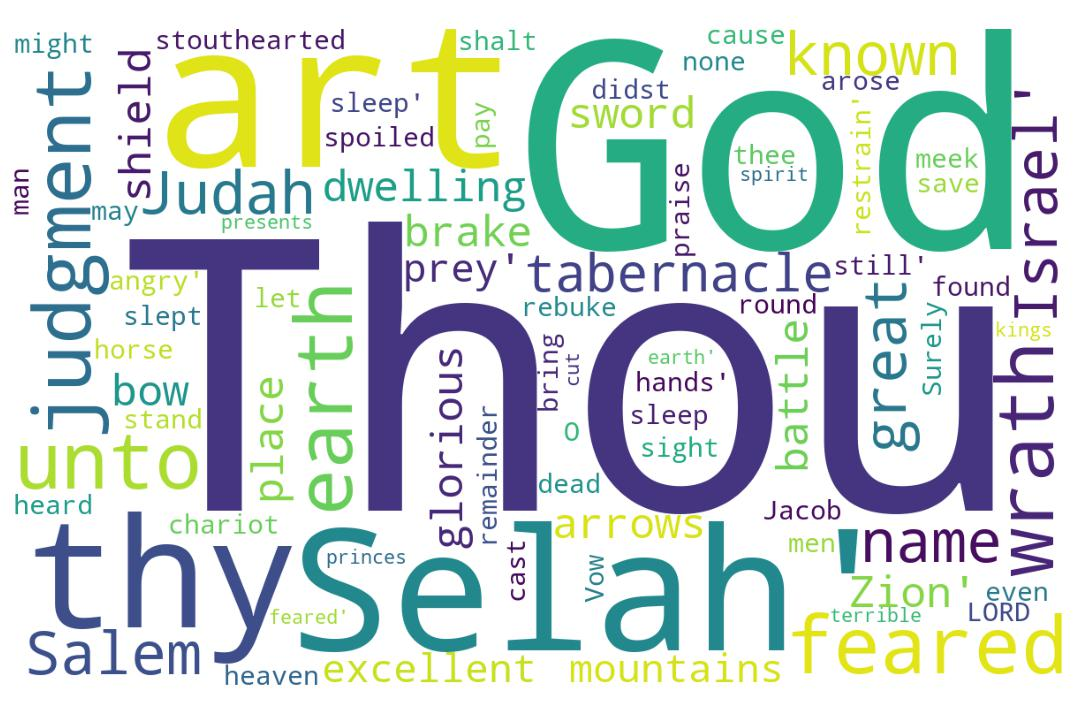
\includegraphics[width=\linewidth]{19OT-Psalms/Psalm76-WordCloud.jpg}
  \caption{Psalm 76 Word Cloud}
  \label{fig:Psalm 76 word Cloud}
\end{figure}

\marginpar{\scriptsize \centering \fcolorbox{bone}{lime}{\textbf{TWO KINDS OF PEOPLE}}\\ (Psalm 76:1-12) \begin{compactenum}[I.][8]
     \item Those \textbf{Shielded} \index[scripture]{Psalms!Psa 076:03}(Psa 76:3)
    \item Those \textbf{Spoiled} \index[scripture]{Psalms!Psa 076:05}(Psa 76:5)
    \item Those \textbf{Put to Sleep} \index[scripture]{Psalms!Psa 076:06}(Psa 76:6)
    \item Those \textbf{Seen} \index[scripture]{Psalms!Psa 076:07}(Psa 76:7)
    \item Those \textbf{Stilled} \index[scripture]{Psalms!Psa 076:08}(Psa 76:8)
    \item Those \textbf{Subdued} \index[scripture]{Psalms!Psa 076:08}(Psa 76:8)
    \item Those \textbf{Saved} \index[scripture]{Psalms!Psa 076:09}(Psa 76:9)
\end{compactenum}}
    




% \textcolor[cmyk]{0.99998,1,0,0}{
\footnote{\textcolor[rgb]{0.00,0.25,0.00}{\hyperlink{TOC}{Return to end of Table of Contents.}}}\footnote{\href{https://audiobible.com/bible/psalms_76.html}{\textcolor[cmyk]{0.99998,1,0,0}{Psalm 76 Audio}}}\textcolor[cmyk]{0.99998,1,0,0}{To the chief Musician on Neginoth, A Psalm \emph{or} Song of Asaph.}\\
\\
\textcolor[cmyk]{0.99998,1,0,0}{In Judah \emph{is} God known: his name \emph{is} great in Israel.} %\footnote{[RUCKMAN] The Psalm is on the Second Advent. God is not known in Judah now, nor has His ``name'' been ``great in Israel'' for 1,950 years. The name “Jehovah” may be great in Israel now, but if we are to believe Deuteronomy 32:15--22; Mark 7:3--13; and Romans 10:1--3, the name is only lip service. God is NOT known, and will not be “known in Judah and Israel” until Hebrews 8:8--12. In this age, God is known, and His “name is great,” among the Gentiles (Acts 28:28), but only because of the Jew (“Judah”). The term “Jew” was given to Judean Jews in Jerusalem (John 5:16, 18), and inspite of tons of anti-Semitic hogwash about “Khazars,” “Edomite usurpers,” and the “ten lost tribes,” salvation is still of the “Jews,” and I don’t mean “Israel” or “the Israel of God” or the “house of Israel.” I mean “Jews,” as in Judean Jews from Judah (vs. 1).\cite{Ruckman1992Psalms}}
[2] \textcolor[cmyk]{0.99998,1,0,0}{In Salem also is his tabernacle, and his dwelling place in Zion.} %\footnote{[RUCKMAN] ``In Salem.” The word is kin to “Shalom” and “Shiloh,” meaning “peace.” God’s dwelling place in this age is NOT in Zion, and He has no tabernacle there; Asaph is prophesying (see the introductory notes). Those who tried to historicize verse 2, and lay it on David or Solomon, have two problems. In the first place, wars do NOT stop in David’s time, nor do they stop in Solomon’s time. The breaking up of weapons in verse 3 is punctuated by our good, old friend “Selah,” showing anyone but a Bible-correcting Hebrew scholar that we are to look at Haggai 2:9 and Zechariah 14 for the meaning of the verse. The word Jerusalem means “city of peace,” so:\cite{Ruckman1992Psalms}
%\begin{compactenum}
%\item It is captured by the Jews in Judges 1:8, but they have to fight against it again to retake it in 2 Samuel 5:6–10. 
%\item Shishak attacks it in 2 Chronicles 12:9.
%\item Jehoash goes after it in 2 Kings 14:13, Rezin in 2 Kings 16:5, and Sennacherib in Isaiah 36 and 37.
%\end{compactenum} 
%Nebuchadnezzar goes up to it three times; Ptolemy Soter attacks it in 320 B.C., Antiochus defiles it in 203 B.C., Scopus attacks it in 199 B.C., and Antiochus hits it again in 168 B.C., and then again “for good measure” in 162 B.C. “City of Peace.” Fantastic, isn’t it? Imagine the commentators thinking that God stopped all the wars with the destruction of David’s foes or Solomon’s or even Hezekiah’s foes (Sennacherib)! Kroll is as tongue tied when he stares at the passage as a calf looking at a “new gate.” He doesn’t know what on earth to do with it. Hyracannus attacks Jerusalem in 65 B.C. Pompey follows suit in 63 B. C. Herod does a bang up job in 39 B.C., and then Titus finishes it off in A.D. 70. But the best is yet to come. Chosroes the Persian attacks it in A.D. 559 after the Romans did it in A.D. 135. Then Afdal takes it in A.D. 1098, after Omar destroyed it in A.D. 637. Then the Crusaders take it (A.D. 1099) only to lose it to Saladin (A.D. 1187). Never fear. Allenby “liberated” it in A.D. 1917, and then the Arabs took over fighting against it with Lebanese, Egyptians, the PLO, the Pope, and the American news media to help them out.\cite{Ruckman1992Psalms}}
[3] \textcolor[cmyk]{0.99998,1,0,0}{There brake he the arrows of the bow, the \fcolorbox{bone}{lime}{shield}, and the sword, and the battle. Selah.}
[4] \textcolor[cmyk]{0.99998,1,0,0}{Thou \emph{art} more glorious \emph{and} excellent than the mountains of prey.} %\footnote{[RUCKMAN] The “thou” is Mt. Zion (see Ps. 68:15 and comments). Two thoughts are present. Mountains which have wild animals on them who take “prey” (Song of Sol. 4:8), are not to be compared with a mountain like Mt. Zion, which not only had the temple on the place where God ordained sacrifices to be made, but also was the location of the Ark of the Covenant which held the Book (Deut. 31:26). The “oracle” of God (1 Kings 6:5) was located on Mt. Zion. The second thought is that the earthly powers represented by mountains (see Rev. 17, for example, and Jeremiah 51:25) are no equal for the “mountain of the Lord” (see Isa. 2:2). He is “king of the mountain,” and His “mountain” will tower above McKinley, Blanc, Whitney, Ararat, Everest, etc., for its prototype (see Heb. 12:22) is already a good bit higher than the entire Milky Way.\cite{Ruckman1992Psalms}}
[5] \textcolor[cmyk]{0.99998,1,0,0}{The stouthearted are \fcolorbox{bone}{lime}{spoiled}, they have slept their sleep: and none of the men of might have found their hands.} %\footnote{[RUCKMAN] Literally, in the sense of Saul (1 Sam. 26:12), who is a type of the Antichrist; doctrinally, in the sense of being dead (see Isa. 26:14; Dan. 12:2). Several things happen at Armageddon that the prophetic expositors never picked up. One of them is that the Antichrist’s troops will kill each other (Judg. 7:22), their flesh will rot on their faces (Zech. 14:12), and their horses will go blind and rabid in the midst of the attack (Zech. 12:4). These are the UN troops (Rev. 19:19) who hope to overthrow the rider on the “white horse” (Rev. 19:10-–14). Observe the advanced revelation found in the AV text which all of the commentators (naturally) missed. When Kroll sees that the “chariot” goes into a dead sleep, as well as the “horses” he mumbles, “the cavalries of the oppressors were stopped.” (Yeah, sonny, they sure were.) The New Idiotic Version (NIV) can’t handle it, so they say that “they lie still.” The Living Baboon says “fell.” The RSV, NRSV, NNRSV (and NNNRSV) take the word “chariot” clean out of the text so they don’t have to deal with the problem: “Both rider and horse lay stunned.” Typical. Absolutely typical of the brand of scholarship you would get at Bob Jones or Liberty University. \cite{Ruckman1992Psalms}}
[6] \textcolor[cmyk]{0.99998,1,0,0}{At thy rebuke, O God of Jacob, both the chariot and horse are cast into a \fcolorbox{bone}{lime}{dead sleep}.} %\footnote{[RUCKMAN] But after 1910, the “chariot” could go to “sleep.” What auto mechanic doesn’t know that? As a matter of fact, the motor can even “die,” and what driver didn’t know that? If it is “awake” but not moving, it is “idling,” and who didn’t know that but the commentators who couldn’t imagine chariots going to sleep? They went to sleep on the Russian front (1942--1944) because the tank fluids froze, or the rats shortcircuited the controls by chewing through the insulation. In my generation (1921--1949), we called automobiles by a peculiar name; we called them “chariots.” A chariot can “malfunction.”\cite{Ruckman1992Psalms}}
[7] \textcolor[cmyk]{0.99998,1,0,0}{Thou, \emph{even} thou, \emph{art} to be feared: and who may stand \fcolorbox{bone}{lime}{in thy sight} when once thou art angry?}
[8] \textcolor[cmyk]{0.99998,1,0,0}{Thou didst cause judgment to be heard from heaven; the earth feared, and was \fcolorbox{bone}{lime}{still}.}
[9] \textcolor[cmyk]{0.99998,1,0,0}{When God arose to judgment, to \fcolorbox{bone}{lime}{save} all the meek of the earth. \fcolorbox{bone}{red}{\textcolor{white}{Selah}}.} %\footnote{[RUCKMAN] All is clear. God “arises” in verse 9 (see Ps. 3:7, 7:6, and 9:19), and not one time is this a reference to God helping anyone out between 500 B. C. and A.D. 2002. “Selah” comes to our aid again to give us the key for judging the critics of the Book. It is a “handy reference” to use in throwing out 80 percent of the rubbish on the Psalms published by Zondervan, Baker, Eerdmans, and Bob Jones University Press. Verse 11 is the exact match for the comments under Psalm 68:29--32, which see. The “vow” of verse 11 is the exact millennial match to Psalm 65:1 and Psalm 50:14, which see. Verse 12 is Armageddon fulfilled, as in Psalm 2:2, 89:27, and Isaiah 24:21. This is a literal destruction at the Advent. In verse 8, we learn that the earth has more sense than most of its inhabitants. The judgment is “heard from heaven,” literally, in Hebrews 12:25; Haggai 2:6; and Psalm 50:3--5 (which see). All of the commentators miss all the references. (This is just as natural for them as breathing.) Note “the meek” of the Sermon on the Mount (Matt. 5:5), showing up in verse 9. \cite{Ruckman1992Psalms}}
[10] \textcolor[cmyk]{0.99998,1,0,0}{Surely the wrath of man shall praise thee: the remainder of wrath shalt thou restrain.} %\footnote{[RUCKMAN ]The destructive critics of the AV come apart at verse 10, which stands in the AV as clear as crystal. The idea is that man’s hatred against God and God’s people will be turned backwards, so that instead of destroying God’s people or stopping God’s hand, God “banks it off the siderail”—He winds up getting glory from it (see Exod. 14:4; Rom. 11:30–34; and Exod. 9:16, 18:11). “The remainder” is a reference to any wrath that does not produce praise for God or glory to Him. Cases are too numerous to mention, the main ones being men killing each other over religious and political issues to the tune of 80,000,000 casualties since A.D. 70. Individual murders (five a day in Detroit, one a day in Las Vegas, two a day in Miami, and ten a day in Washington, D.C.) do not praise God, but murderers are restrained so that total mayhem and murder don’t break out internationally with five hundred killed daily in Memphis, Atlanta, London, Paris, New York, Rome, Madrid, Tokyo, Bombay, Athens, Oslo, Seattle, and Oklahoma City. What wrath does not praise God is held in check so it doesn’t annihilate mankind altogether. Today the Arabs are restrained by “the restrainer” (2 Thess. 2:6–7); otherwise, they would have pushed Israel off into the Mediterranean more than sixty years ago. Kroll (LU) can’t handle it. His peers (Falwell and company) printed a NKJV that reads “you shall gird yourself.” But having made this change, in line with most “highly qualified, recognized Hebrew scholarship” available--used in the RSV, NRSV, and NIV-- they are powerless to interpret the mess they produced, so they leave it there like a rotten egg and print the AV text in the commentary, and then refuse to comment on it! Liberty University inherited its corruption from Edward Wetenhall, the Lord Bishop of Corke and Rosse (1661), Cornelius Buges (1614), and Maurer. These gentlemen tell us that “the Hebrew says....” (Oh, don’t you know. Don’t you just know “the Hebrew says.” I know what “the Hebrew says.” It says whatever the Cult wants you to think it should say. You don’t fool me, kiddies. I used to bartend and lifeguard for a living. You don’t fool me. I’ve shot craps in the alley, played poker “below decks,” got drunk in the French Quarter, and played “cops and teen agers” at all hours of the night. Don’t kid me. I know what the “Hebrew” better say, even if it doesn’t say it.) “Probably it is meant that God girds himself with the praise to which the last of the enemy even to its last remnant is constrained to minister, both in the case of reprobates and....” Yep; that is exactly what it didn’t say, and that is exactly what it didn’t mean. “This, in the Hebrew, is expressed in one word...which imports the begirding or binding of it on every side, that it shall by no means break out, but shall be kept in, as a dog on a chain....” Oh, I got it! He is “held in restraint”! He is a “restrainer”; a leash. Oh yeah, I got “the Hebrew” now! It didn’t mean “gird” at all. It meant “the remainder of wrath shalt thou restrain.” (That’s what I thought you said.) The Living Bible says the “remainder” is an “ornament,” and the Nitty Ickey Version (NIV) says that some “survivors” of God’s wrath are restrained. In the Asinine Standard Vision (ASV), God girds Himself with wrath that came from men instead of Himself. Ditto the Rotten Stupid Version (RSV). Stupidity is infectious. It is passed reverently from one generation of “godly” men to another, so that “historic positions” can overthrow the truth of God in each generation. \cite{Ruckman1992Psalms} }
[11] \textcolor[cmyk]{0.99998,1,0,0}{Vow, and pay unto the LORD your God: let all that be round about him bring presents unto him that ought to be feared.} %\footnote{[RUCKMAN] The ``earth feared'' because the Lord is the One ``that ought to be feared'' (vs. 11). This is for a number of reasons:\cite{Ruckman1992Psalms}
%\begin{compactenum}
%\item He will break all your weapons of war in pieces no matter how “advanced” they are.
%\item He can cast you into a deep sleep (Acts 12:6; Matt. 25:5) when you need to be awake.
%\item He will cut off world rulers, in terror, even if they are ``kings'' and ``princes.''
%\item He can cast you out of His sight and destroy both body and soul in Hell (Matt. 10:28).
%\end{compactenum}}
[12] \textcolor[cmyk]{0.99998,1,0,0}{He shall cut off the spirit of princes: \emph{he} \emph{is} terrible to the kings of the earth.}

\chapter{Proverb 17}
\begin{figure}
  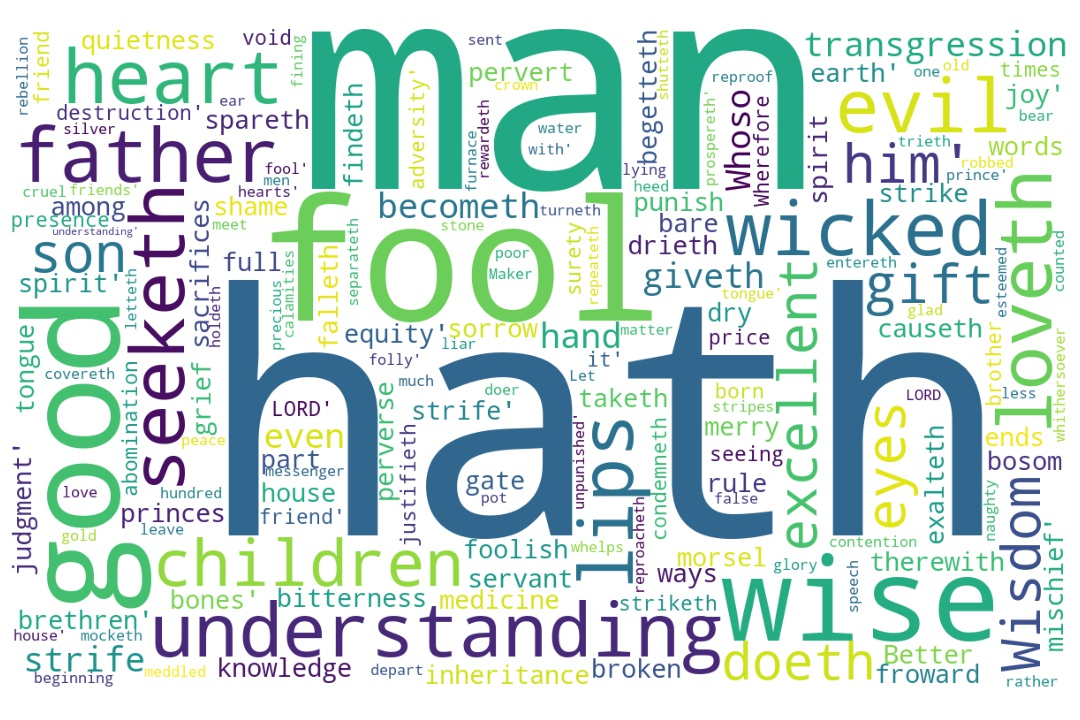
\includegraphics[width=\linewidth]{20OT-Proverbs/Proverb17-WordCloud.jpg}
  \caption{Proverb 17 Word Cloud}
  \label{fig:Proverb 17 word Cloud}
\end{figure}

\marginpar{\scriptsize \centering \fcolorbox{bone}{lime}{\textbf{CONTRASTS}}\\ (Proverbs 17:1-28) \begin{compactenum}[I.][8]
    \item \textbf{A Dry Morsel} \index[scripture]{Proverbs!Pro 17:01}(Pro 17:1) 
    \item \textbf{A Dim-Witted Mocker} \index[scripture]{Proverbs!Pro 17:05}(Pro 17:5) 
    \item \textbf{A Divisive Matter} \index[scripture]{Proverbs!Pro 17:09}(Pro 17:9) 
    \item \textbf{A Disruptive Messenger} \index[scripture]{Proverbs!Pro 17:11}(Pro 17:11) 
    \item \textbf{Destructive Meddling} \index[scripture]{Proverbs!Pro 17:14}(Pro 17:14) 
    \item \textbf{Dangerous Mischief} \index[scripture]{Proverbs!Pro 17:20}(Pro 17:20) 
    \item \textbf{A Discerning Man} \index[scripture]{Proverbs!Pro 17:28} (Pro 17:28) 
\end{compactenum} }

\marginpar{\scriptsize \centering \fcolorbox{bone}{yellow}{\textbf{THE FRUIT OF FOOLS}}\\ (Proverbs 17:1-28) \begin{compactenum}[I.][8]
    \item \textbf{Unwanted Family} \index[scripture]{Proverbs!Pro 17:01}(Pro 17:1) 
    \item \textbf{Unteachable Fool} \index[scripture]{Proverbs!Pro 17:10}(Pro 17:10) 
    \item \textbf{Unstoppable Fool} \index[scripture]{Proverbs!Pro 17:11}(Pro 17:11)  
    \item \textbf{Unrestrained Fanatic} \index[scripture]{Proverbs!Pro 17:11}(Pro 17:11)
    \item \textbf{Uncontrollable Flood} \index[scripture]{Proverbs!Pro 17:14}(Pro 17:14)  
    \item \textbf{Unshakeable Fealty} \index[scripture]{Proverbs!Pro 17:17}(Pro 17:17)  
    \item \textbf{Unfulfilled Father} \index[scripture]{Proverbs!Pro 17:21}(Pro 17:21) 
    \item \textbf{Unobtainable Focus} \index[scripture]{Proverbs!Pro 17:24}(Pro 17:24)  
\end{compactenum} }

\footnote{\textcolor[cmyk]{0.99998,1,0,0}{\hyperlink{TOC}{Return to end of Table of Contents.}}}\footnote{\href{https://audiobible.com/bible/proverbs_17.html}{\textcolor[cmyk]{0.99998,1,0,0}{Proverbs Audio}}}\textcolor[cmyk]{0.99998,1,0,0}{Better \emph{is} a \fcolorbox{bone}{lime}{dry morsel}, and quietness therewith, than an house full of sacrifices \emph{with} strife.}
[2] \textcolor[cmyk]{0.99998,1,0,0}{A wise servant shall have rule over a son that causeth shame, and shall have part of the inheritance among the brethren.}
[3] \textcolor[cmyk]{0.99998,1,0,0}{The fining pot \emph{is} for silver, and the furnace for gold: but the LORD trieth the hearts.}
[4] \textcolor[cmyk]{0.99998,1,0,0}{A wicked doer giveth heed to false lips; \emph{and} a liar giveth ear to a naughty tongue.}
[5] \textcolor[cmyk]{0.99998,1,0,0}{Whoso \fcolorbox{bone}{lime}{mocketh} the poor reproacheth his Maker: \emph{and} he that is glad at calamities shall not be unpunished.}
[6] \textcolor[cmyk]{0.99998,1,0,0}{Children's children \emph{are} the crown of old men; and the glory of children \emph{are} their fathers.}
[7] \textcolor[cmyk]{0.99998,1,0,0}{Excellent speech becometh not a fool: much less do lying lips a prince.}
[8] \textcolor[cmyk]{0.99998,1,0,0}{A gift \emph{is} \emph{as} a precious stone in the eyes of him that hath it: \fcolorbox{bone}{MYGOLD}{whithersoever} it turneth, it prospereth.}
[9] \textcolor[cmyk]{0.99998,1,0,0}{He that covereth a \fcolorbox{bone}{MYGOLD}{transgression} seeketh love; but he that repeateth a matter \fcolorbox{bone}{lime}{separateth} \emph{very} friends.}
[10] \textcolor[cmyk]{0.99998,1,0,0}{A reproof entereth more into a wise man than an hundred stripes into a fool.}
[11] \textcolor[cmyk]{0.99998,1,0,0}{An evil \emph{man} seeketh only rebellion: therefore a \fcolorbox{bone}{lime}{cruel messenger} shall be sent against him.}
[12] \textcolor[cmyk]{0.99998,1,0,0}{Let a bear robbed of her whelps meet a man, rather than a fool in his folly.}
[13] \textcolor[cmyk]{0.99998,1,0,0}{Whoso rewardeth evil for good, evil shall not depart from his house.}
[14] \textcolor[cmyk]{0.99998,1,0,0}{The beginning of strife \emph{is} \emph{as} when one letteth out water: therefore leave off contention, before it be \fcolorbox{bone}{lime}{meddled} with.}
[15] \textcolor[cmyk]{0.99998,1,0,0}{He that justifieth the wicked, and he that condemneth the just, even they both \emph{are} abomination to the LORD.}
[16] \textcolor[cmyk]{0.99998,1,0,0}{Wherefore \emph{is} \emph{there} a price in the hand of a fool to get wisdom, seeing \emph{he} \emph{hath} no heart \emph{to} \emph{it}?}
[17] \textcolor[cmyk]{0.99998,1,0,0}{A friend loveth at all times, and a brother is born for adversity.}
[18] \textcolor[cmyk]{0.99998,1,0,0}{A man void of \fcolorbox{bone}{MYGOLD}{understanding} striketh hands, \emph{and} becometh surety in the presence of his friend.}
[19] \textcolor[cmyk]{0.99998,1,0,0}{He loveth \fcolorbox{bone}{MYGOLD}{transgression} that loveth strife: \emph{and} he that exalteth his gate seeketh destruction.}
[20] \textcolor[cmyk]{0.99998,1,0,0}{He that hath a froward heart findeth no good: and he that hath a perverse tongue falleth into \fcolorbox{bone}{lime}{mischief}.}
[21] \textcolor[cmyk]{0.99998,1,0,0}{He that begetteth a fool \emph{doeth} \emph{it} to his sorrow: and the father of a fool hath no joy.}
[22] \textcolor[cmyk]{0.99998,1,0,0}{A merry heart doeth good \emph{like} a medicine: but a broken spirit drieth the bones.}
[23] \textcolor[cmyk]{0.99998,1,0,0}{A wicked \emph{man} taketh a gift out of the bosom to pervert the ways of judgment.}
[24] \textcolor[cmyk]{0.99998,1,0,0}{Wisdom \emph{is} before him that hath \fcolorbox{bone}{MYGOLD}{understanding}; but the eyes of a fool \emph{are} in the ends of the earth.}
[25] \textcolor[cmyk]{0.99998,1,0,0}{A foolish son \emph{is} a grief to his father, and bitterness to her that bare him.}
[26] \textcolor[cmyk]{0.99998,1,0,0}{Also to punish the just \emph{is} not good, \emph{nor} to strike princes for equity.}
[27] \textcolor[cmyk]{0.99998,1,0,0}{He that hath knowledge spareth his words: \emph{and} a man of \fcolorbox{bone}{MYGOLD}{understanding} is of an excellent spirit.}
[28] \textcolor[cmyk]{0.99998,1,0,0}{Even a fool, when he holdeth his peace, is counted wise: \emph{and} he that shutteth his lips \emph{is} \emph{esteemed} \fcolorbox{bone}{lime}{a man of \fcolorbox{bone}{MYGOLD}{understanding}}.}




\end{document}

